\documentclass[../main.tex]{subfiles}

\begin{document}

\section*{第1問}

\begin{proof}[解]
\textbf{(1)} $Q(\alpha,\alpha^2)$，$R(\beta,\beta^2)$（$\alpha<\beta$）とおいて良い。この時$Q,R$での接線は各々
\[
y=2\alpha x-\alpha^2, \qquad y=2\beta x-\beta^2
\]
だから，$P$はこの交点で，$\left(\dfrac{\alpha+\beta}{2},\alpha\beta\right)$である。$P$は$y=x^2$の下側だから，
\[
\alpha\beta<\frac14(\alpha+\beta)^2 \quad\therefore\ (\alpha-\beta)^2>0
\]
これは$\alpha<\beta$から常にみたされる。そこで，$\alpha,\beta$が，$A=\alpha+\beta,\ b=\alpha\beta$とした時，実数解条件及び題意から
\[
b\le\frac12A-1,\ -\frac12A+1 \quad\cdots\text{①}
\]
\[
-1\le b,\quad b\le\frac14A^2
\]
をみたしながら動く時のQRの中点$M(X,Y)$の軌跡を求めれば良い。
\[
X=\frac12(\alpha+\beta)=\frac12A \quad\cdots\text{②}
\]
\[
Y=\frac12(\alpha^2+\beta^2)=\frac12(A^2-2b)
\]
であり，①を図示すると右図斜線部（境界含む）だから，
\[
-1\le b\le\frac12A-1 \quad(0\le A\le2) \quad\cdots\text{③}
\]
\[
-1\le b\le-\frac12A+1 \quad(2\le A\le4)
\]
②③から
\[
\frac12A^2-\frac12A+1\le Y\le\frac12A^2+1 \quad(0\le A\le2) \quad\cdots\text{④}
\]
\[
\frac12A^2+\frac12A-1\le Y\le\frac12A^2+1 \quad(2\le A\le4)
\]
④に②を代入して
\[
2X^2-X+1\le Y\le2X^2+1 \quad(0\le X\le1)
\]
\[
2X^2+X-1\le Y\le2X^2+1 \quad(1\le X\le2)
\]
これがもとめる領域で，図示して下図斜線部。

\begin{center}
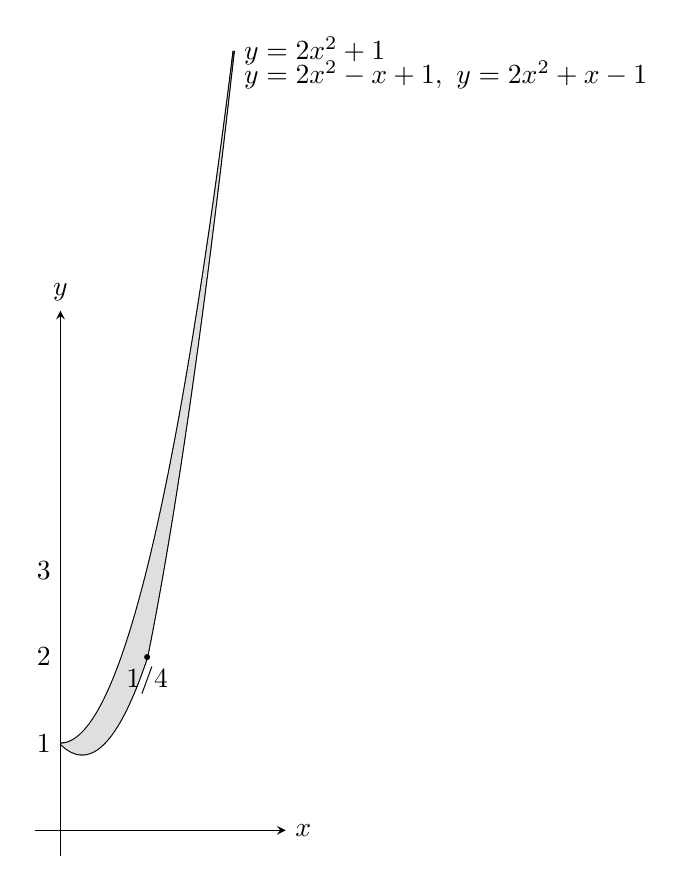
\begin{tikzpicture}[scale=1.1, >=stealth]
  \draw[->] (-0.3,0) -- (2.6,0) node[right] {$x$};
  \draw[->] (0,-0.3) -- (0,6) node[above] {$y$};
  \draw[domain=0:2, smooth, thick] plot (\x,{2*\x*\x+1}) node[right] {$y=2x^2+1$};
  \draw[domain=0:1, smooth, thick] plot (\x,{2*\x*\x-\x+1});
  \draw[domain=1:2, smooth, thick] plot (\x,{2*\x*\x+\x-1}) node[below right] {$y=2x^2-x+1,\ y=2x^2+x-1$};
  \fill[gray!25, domain=0:1, variable=\x] plot ({\x},{2*\x*\x+1}) -- plot[domain=1:0] ({\x},{2*\x*\x-\x+1}) -- cycle;
  \fill[gray!25, domain=1:2, variable=\x] plot ({\x},{2*\x*\x+1}) -- plot[domain=2:1] ({\x},{2*\x*\x+\x-1}) -- cycle;
  \fill (1,2) circle (1pt) node[below] {$1/4$};
  \node[left] at (0,3) {$3$};
  \node[left] at (0,2) {$2$};
  \node[left] at (0,1) {$1$};
\end{tikzpicture}
\end{center}

\textbf{(2)}
\[
\overrightarrow{PQ}=\left(\alpha-\frac{\alpha+\beta}{2},\ \alpha^2-\alpha\beta\right)=\left(\frac{\alpha-\beta}{2},\ \alpha(\alpha-\beta)\right)
\]
\[
\overrightarrow{PR}=\left(\beta-\frac{\alpha+\beta}{2},\ \beta^2-\alpha\beta\right)=\left(\frac{\beta-\alpha}{2},\ \beta(\beta-\alpha)\right)
\]
だから，サラスの公式から，
\[
\triangle PQR=\frac12\left|\frac12(\alpha-\beta)\beta(\beta-\alpha)-\frac12(\beta-\alpha)\alpha(\alpha-\beta)\right|=\frac14(\beta-\alpha)^3 \quad(\because\beta>\alpha) \quad\cdots\text{⑤}
\]
ここで，$\beta,\alpha$は$t$の2次式$t^2-at+b=0$の2実解で$t=\dfrac{a\pm\sqrt{a^2-4b}}{2}$でかつ$\alpha<\beta$から
\[
\beta-\alpha=\sqrt{a^2-4b} \quad\cdots\text{⑥}
\]
なので，⑥を⑤に代入して，
\[
\triangle PQR=\frac14(a^2-4b)^{\frac32}
\]
$\triangle PQR=2$の時，
\[
8=(a^2-4b)^{\frac32} \iff 4=a^2-4b \quad(\because a^2-4b>0)
\]
だから，$P(X,Y)$について$X=\dfrac12a,\ Y=b$だから，
\[
Y=X^2-1
\]
である。
\end{proof}

\newpage

\section*{第2問}

\begin{proof}[解]
$A: x^2+y^2=4$，$B_0: (x-3)^2+y^2=1$とおく。$B_0$の中心$C_0$，$B$の中心$C$，$A$と$B$の接点を$D$とおく。$\angle DOC_0=\theta$（$0\le\theta\le2\pi$）の時，弧長$=2\theta$（$P_0\to P$まで，$A$と接していた方の弧）だから，$\angle PCD$（弧度を含む方）$=2\theta$であり，$P$の座標$P(X,Y)$は
\[
\begin{pmatrix}X\\Y\end{pmatrix}=\overrightarrow{OC}+\overrightarrow{CP}=3\begin{pmatrix}\cos\theta\\\sin\theta\end{pmatrix}+\begin{pmatrix}\cos(3\theta-\pi)\\\sin(3\theta-\pi)\end{pmatrix}=3\begin{pmatrix}C\\S\end{pmatrix}-\begin{pmatrix}\cos3\theta\\\sin3\theta\end{pmatrix}
\]
とかける（$C=\cos\theta,\ S=\sin\theta$）。
\[
\frac{dX}{d\theta}=-3S+3(3S-4S^3)=3S(2-4S^2)
\]
\[
\frac{dY}{d\theta}=3C-3(4C^3-3C)=3C(4-4C^2)
\]
から下表をうる。ただし，$\left.\begin{pmatrix}X\\Y\end{pmatrix}\right|_{\theta=t}$と$\left.\begin{pmatrix}X\\Y\end{pmatrix}\right|_{\theta=2\pi-t}$（$0\le t\le\pi$）が$x$軸に関して対称なので，$0\le\theta\le\pi$とした。
\begin{center}
\begin{tabular}{c|ccccccccc}
$\theta$ & $0$ & & $\frac{\pi}{4}$ & & $\frac{\pi}{2}$ & & $\frac{3}{4}\pi$ & & $\pi$ \\
\hline
$X'$ & $+$ & $+$ & $0$ & $-$ & $-$ & $-$ & $0$ & $+$ & \\
\hline
$Y'$ & $+$ & $+$ & $+$ & $0$ & $-$ & $-$ & $-$ & $-$ & \\
\hline
$(X,Y)$ & $(2,0)$ & $\nearrow$ & $(2\sqrt2,\sqrt2)$ & $\nwarrow$ & $(0,4)$ & $\swarrow$ & $(-2\sqrt2,\sqrt2)$ & $\searrow$ & $(-2,0)$
\end{tabular}
\end{center}
したがって，$C$（曲線）で$x$座標が最大なのは，$(2\sqrt2,\pm\sqrt2)$である。

又，$C$の長さを$L$として，$(X,Y)$が$x$軸についても対称なことから，
\[
\frac{L}{4}=\int_0^{\frac{\pi}{2}}\sqrt{\left[3S(2-4S^2)\right]^2+\left[3C(4-4C^2)\right]^2}\,d\theta
\]
\[
=\int_0^{\frac{\pi}{2}}\sqrt{36S^2(1-2S^2)^2+144C^2S^4}\,d\theta
\]
\[
=\int_0^{\frac{\pi}{2}}\sqrt{36\sin^2\theta}\,d\theta
\]
\[
=\int_0^{\frac{\pi}{2}}6\sin\theta\,d\theta \quad(\because\sin\theta\ge0)
\]
\[
=6\left[-\cos\theta\right]_0^{\frac{\pi}{2}}=6
\]
\[
L=24
\]
\end{proof}

\newpage

\section*{第3問}

\begin{proof}[解]
\[
f(x+y)=f(x)+f(y)+f(x)f(y) \quad\cdots\text{①}
\]

\textbf{(1)}
\[
\frac{f(x+y)-f(x)}{y}=\frac{f(y)(1+f(x))}{y}\longrightarrow f'(0)(1+f(x)) \quad(y\to0)
\]
より示すべきことは明らか。$\blacksquare$

\textbf{(2)} $a=f'(0)$とおく。まず①で$(x,y)=(0,0)$として，
\[
f(0)(1+f(0))=0 \quad\therefore\ f(0)=0,-1 \quad\cdots\text{②}
\]
である。(1)から，$y=f(x)$とおくと，
\[
\frac{dy}{dx}=a(1+y) \quad\cdots\text{③}
\]
$a=0$の時，$y=C$（$C$：定数）とおける。①に代入して$C=0$だから，$f(x)=0$は解の1つ。以下$a\ne0$とする。③から
\[
\frac{dy}{1+y}=a\,dx
\]
積分して
\[
\log(1+y)=ax+C_1
\]
\[
y=C\cdot e^{ax}-1
\]
とおける。ただし，$C,C_1$は定数。②に代入して，$C=0,1$である。

\textbf{$1^\circ$ $C=1$の時}

$y=e^{ax}-1$だから，①に代入すると
\[
(\text{左辺})=e^{a(x+y)}-1
\]
\[
(\text{右辺})=e^{ax}+e^{ay}-2+(e^{ax}-1)(e^{ay}-1)=e^{a(x+y)}-1
\]
となって恒等的に①は成立。

\textbf{$2^\circ$ $C=0$の時}

$y=-1$となり，不適（$a\ne0$の仮定に反する）。

以上から
\[
y=0,\quad e^{f'(0)x}-1
\]
\end{proof}

\newpage

\section*{第4問}

\begin{proof}[解]
$I_n=\displaystyle\int_0^\pi x^2|\sin nx|dx$，$a_k=\displaystyle\int_{\frac{k-1}{n}\pi}^{\frac{k}{n}\pi}x^2|\sin nx|dx$，$f(x)=x^2$とし，$\left[\dfrac{k-1}{n}\pi,\dfrac{k}{n}\pi\right]$で$f(x)$の$\max,\min$を与える$x$を$M_k,m_k$とする。$|\sin nx|\ge0$だから，
\[
f(m_k)|\sin nx|\le f(x)|\sin nx|\le f(M_k)|\sin nx|
\]
積分して，
\[
f(m_k)\int_{\frac{k-1}{n}\pi}^{\frac{k}{n}\pi}|\sin nx|dx\le a_k\le f(M_k)\int_{\frac{k-1}{n}\pi}^{\frac{k}{n}\pi}|\sin nx|dx \quad\cdots\text{①}
\]
ここで，$\displaystyle\int_{\frac{k-1}{n}\pi}^{\frac{k}{n}\pi}|\sin nx|dx=\dfrac2n$だから，①から，
\[
\frac2nf(m_k)\le a_k\le\frac2nf(M_k)
\]
$k$について和をとって，
\[
\frac2n\sum_{k=1}^nf(m_k)\le I_n\le\frac2n\sum_{k=1}^nf(M_k) \quad\cdots\text{②}
\]
ここで，区分求積からいずれのものとして
\[
\frac1n\sum_{k=1}^nf(m_k)\longrightarrow\frac1\pi\int_0^\pi f(x)dx=\frac13\pi^2
\]
\[
\frac1n\sum_{k=1}^nf(M_k)\longrightarrow\frac13\pi^2
\]
だから，②及びはさみうちから，
\[
I_n\longrightarrow\frac23\pi^2
\]
\end{proof}

\newpage

\section*{第5問}

\begin{proof}[解]
\[
\begin{array}{ccc}
k-1 & \xrightarrow{1-\frac{k-1}{n}} & k \\
r-1 & & r \\
r & \xrightarrow{\frac{r}{n}} & r
\end{array}
\]

\textbf{(1)} 上図から
\[
P(S_k=r)=\frac{n+1-r}{n}P(S_{k-1}=r-1)+\frac{r}{n}P(S_{k-1}=r) \quad(r=1,2,\cdots,k\text{の時}, P(S_0=r)=0\text{と扱う})
\]

\textbf{(2)} 確率変数$X_t$を，
\[
X_t=
\begin{cases}
0 & (t\text{のカードを}k\text{回目まで引かなかった}) \\
1 & (t\text{のカードを}k\text{回目までに引いた})
\end{cases}
\]
と定めると，$S_k=\displaystyle\sum_{t=1}^nX_t$だから，期待値の加法性から
\[
E(S_k)=E\left(\sum_{t=1}^nX_t\right)=\sum_{t=1}^nE(X_t)=nE(X_1) \quad(\because\text{対称性}) \quad\cdots\text{①}
\]
である。$k$回目までに1のカードを引く確率$\ell_k$は，排反をかんがえて，
\[
\ell_k=1-\left(\frac{n-1}{n}\right)^k
\]
で，$E(X_1)=0\cdot P(X_1=0)+1\cdot P(X_1=1)=P(X_1=1)=\ell_k$だから，①より，
\[
E_k=n\left[1-\left(\frac{n-1}{n}\right)^k\right]
\]
\end{proof}

\bigskip
\noindent\textbf{[別解]}

\begin{proof}[別解]
\textbf{(2)} (1)の両辺$r$をかけて$r$について和をとる。
\[
\sum_{r=1}^krP(S_k=r)=\sum_{r=1}^k\frac{r^2}{n}P(S_{k-1}=r)+\sum_{r=1}^k\frac{nr+r(r-1)}{n}P(S_{k-1}=r-1)
\]
$P(S_{k-1}=k)=0$だから，
\[
E_k=\sum_{r=1}^{k-1}\frac{r^2}{n}P(S_{k-1}=r)+\sum_{r=1}^k\frac{(n-1)(r-1)+n-(r-1)^2}{n}P(S_{k-1}=r-1)
\]
\[
=\sum_{r=1}^{k-1}\frac{r^2}{n}P(S_{k-1}=r)+\frac{n-1}{n}E_{k-1}+\sum_{r=1}^kP(S_{k-1}=r-1)-\sum_{r=1}^k\frac{(r-1)^2}{n}P(S_{k-1}=r-1)
\]
最初の和と最後の和は（添字を$j=r-1$とおきかえると）互いに打ち消しあうので，$\displaystyle\sum_{r=1}^kP(S_{k-1}=r-1)=1$から，
\[
E_k=\frac{n-1}{n}E_{k-1}+1
\]
だから，$E_1=1$より
\[
E_k=n\left[1-\left(\frac{n-1}{n}\right)^k\right]
\]
\end{proof}

\end{document}
